\chapter{Mathematical Logic, Proof Methods \& Set Theory}
\label{chap:logic_sets}

\section{Propositional Logic and Logical Connectives}

Mathematical analysis is built upon the foundation of formal logic. A \textbf{mathematical assertion} (or proposition) is a declarative statement that is unambiguously either \textbf{True} ($\mathrm{T}$ or $1$) or \textbf{False} ($\mathrm{F}$ or $0$), but never both simultaneously (the \textit{Law of Excluded Middle} and the \textit{Principle of Non-Contradiction}).

\begin{figure}[htbp]
  \centering
  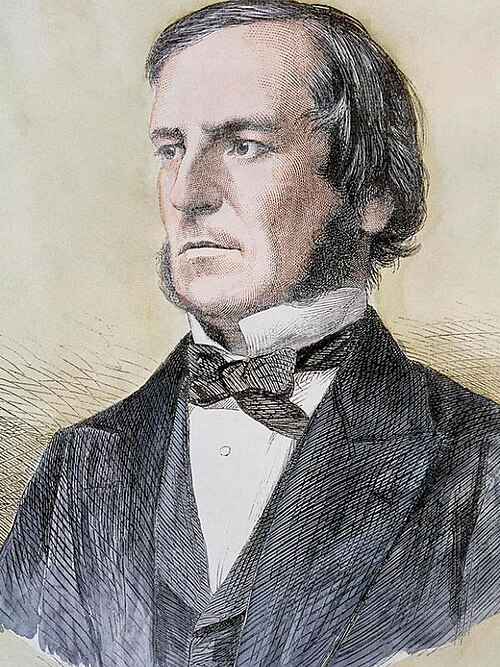
\includegraphics[width=0.28\textwidth]{boole.jpg}
  \caption{\textbf{George Boole (1815--1864)}, English mathematician and philosopher who formalized symbolic mathematical logic in \textit{The Laws of Thought} (1854), laying the algebraic foundation of modern computing and formal mathematics.}
  \label{fig:boole}
\end{figure}

\begin{definitionbox}{Elementary Logical Connectives}
Let $P$ and $Q$ be two propositions. We define compound propositions via truth functions:
\begin{enumerate}[leftmargin=1.4em,itemsep=3pt]
  \item \textbf{Negation ($\neg P$ or $\overline{P}$):} "Not $P$". True if and only if $P$ is false.
  \item \textbf{Conjunction ($P \land Q$):} "$P$ and $Q$". True if and only if both $P$ and $Q$ are simultaneously true.
  \item \textbf{Disjunction ($P \lor Q$):} "$P$ or $Q$" (inclusive or). True if at least one of $P$ or $Q$ is true; false only if both are false.
  \item \textbf{Implication ($P \implies Q$):} "$P$ implies $Q$" or "If $P$, then $Q$". False if and only if $P$ is true and $Q$ is false. By definition, $P \implies Q$ is logically equivalent to $(\neg P) \lor Q$.
  \item \textbf{Equivalence ($P \iff Q$):} "$P$ is equivalent to $Q$" or "$P$ if and only if $Q$". True if both $P$ and $Q$ possess the same truth value. Logically equivalent to $(P \implies Q) \land (Q \implies P)$.
\end{enumerate}
\end{definitionbox}

\begin{center}
\renewcommand{\arraystretch}{1.25}
\begin{tabular}{ccccccc}
\toprule
$P$ & $Q$ & $\neg P$ & $P \land Q$ & $P \lor Q$ & $P \implies Q$ & $P \iff Q$ \\
\midrule
$\mathrm{T}$ & $\mathrm{T}$ & $\mathrm{F}$ & $\mathrm{T}$ & $\mathrm{T}$ & $\mathrm{T}$ & $\mathrm{T}$ \\
$\mathrm{T}$ & $\mathrm{F}$ & $\mathrm{F}$ & $\mathrm{F}$ & $\mathrm{T}$ & $\mathrm{F}$ & $\mathrm{F}$ \\
$\mathrm{F}$ & $\mathrm{T}$ & $\mathrm{T}$ & $\mathrm{F}$ & $\mathrm{T}$ & $\mathrm{T}$ & $\mathrm{F}$ \\
$\mathrm{F}$ & $\mathrm{F}$ & $\mathrm{T}$ & $\mathrm{F}$ & $\mathrm{F}$ & $\mathrm{T}$ & $\mathrm{T}$ \\
\bottomrule
\end{tabular}
\end{center}

\begin{propbox}{Essential Tautologies and De Morgan's Logical Laws}
For any propositions $P, Q, R$, the following compound propositions are \textbf{tautologies} (true under all truth assignments):
\begin{enumerate}[leftmargin=1.4em,itemsep=2pt]
  \item \textbf{Double Negation:} $\neg(\neg P) \iff P$.
  \item \textbf{De Morgan's Laws:}
  \[
  \neg(P \land Q) \iff (\neg P) \lor (\neg Q), \qquad \neg(P \lor Q) \iff (\neg P) \land (\neg Q).
  \]
  \item \textbf{Distributivity:}
  \[
  P \land (Q \lor R) \iff (P \land Q) \lor (P \land R), \qquad P \lor (Q \land R) \iff (P \lor Q) \land (P \lor R).
  \]
  \item \textbf{Contrapositive Equivalence (Transposition):}
  \[
  (P \implies Q) \iff (\neg Q \implies \neg P).
  \]
  \item \textbf{Reductio ad Absurdum (Contradiction):}
  \[
  (P \implies Q) \iff \left[ (P \land \neg Q) \implies \text{Contradiction} \right].
  \]
\end{enumerate}
\end{propbox}

\section{Universal and Existential Quantifiers}

In mathematical analysis, assertions typically contain variables evaluated over specified sets. A statement containing a variable $x \in E$ is called an \textbf{open sentence} or \textbf{predicate}, denoted $P(x)$.

\begin{definitionbox}{Quantifiers and Their Scopes}
\begin{enumerate}[leftmargin=1.4em,itemsep=3pt]
  \item \textbf{Universal Quantifier ($\forall$, "for all" / "for every"):}
  \[
  \forall x \in E, \quad P(x)
  \]
  is true if and only if $P(x)$ holds true for every single element $x$ in the domain $E$.
  \item \textbf{Existential Quantifier ($\exists$, "there exists at least one"):}
  \[
  \exists x \in E, \quad P(x)
  \]
  is true if and only if there is at least one element $x \in E$ for which $P(x)$ is true.
  \item \textbf{Uniqueness Quantifier ($\exists!$, "there exists a unique"):}
  \[
  \exists! x \in E, \quad P(x) \iff \left[ (\exists x \in E, P(x)) \land (\forall x, y \in E, (P(x) \land P(y)) \implies x = y) \right].
  \]
\end{enumerate}
\end{definitionbox}

\begin{theorembox}{Negation of Quantified Statements}
The negation of quantified statements swaps the quantifiers and negates the inner predicate:
\begin{align}
\neg \left( \forall x \in E, \ P(x) \right) &\iff \exists x \in E, \ \neg P(x), \\
\neg \left( \exists x \in E, \ P(x) \right) &\iff \forall x \in E, \ \neg P(x).
\end{align}
For multi-quantifier propositions, the order of quantifiers is critical and cannot be arbitrarily exchanged:
\[
\exists y \in F, \ \forall x \in E, \ P(x, y) \implies \forall x \in E, \ \exists y \in F, \ P(x, y),
\]
but the converse is \textbf{false} in general!
\end{theorembox}

\section{Methods of Mathematical Proof}

\begin{enumerate}[leftmargin=1.4em,itemsep=4pt]
  \item \textbf{Direct Proof:} Assume $P$ is true. Through a sequence of rigorous deductions using axioms, definitions, and established theorems, show that $Q$ necessarily follows.
  \item \textbf{Proof by Contrapositive:} To prove $P \implies Q$, we prove the logically equivalent contrapositive statement $\neg Q \implies \neg P$. This is especially powerful when $\neg Q$ provides more concrete algebraic structure than $P$.
  \item \textbf{Proof by Contradiction (\textit{Reductio ad Absurdum}):} To prove an assertion $A$, assume its negation $\neg A$ is true. Derive a logical contradiction (such as $0 = 1$ or $x \in B \land x \notin B$). Therefore, $\neg A$ must be false, establishing that $A$ is true.
  \item \textbf{Disproof by Counterexample:} To disprove a universal assertion $\forall x \in E, P(x)$, it suffices to produce a single concrete element $x_0 \in E$ for which $P(x_0)$ is false.
  \item \textbf{Proof by Mathematical Induction:}
  \begin{theorembox}{Principle of Mathematical Induction (Peano Axiom)}
  Let $P(n)$ be a predicate defined for all integers $n \ge n_0$ ($n_0 \in \mathbb{Z}$). If:
  \begin{enumerate}[leftmargin=1.2em,itemsep=2pt]
    \item \textbf{Base Step:} $P(n_0)$ is true;
    \item \textbf{Inductive Step:} For any arbitrary integer $k \ge n_0$, the assumption that $P(k)$ is true (the \textit{induction hypothesis}) implies that $P(k+1)$ is true:
    \[
    \forall k \ge n_0, \quad P(k) \implies P(k+1);
    \]
  \end{enumerate}
  Then $P(n)$ is true for all integers $n \ge n_0$.
  \end{theorembox}
\end{enumerate}

\section{Axiomatic Set Theory and Operations}

A \textbf{set} is an intuitive collection of well-defined, distinct mathematical objects called its \textbf{elements}. If an object $x$ belongs to a set $A$, we write $x \in A$; otherwise $x \notin A$.

\begin{definitionbox}{Subsets, Equality, and the Power Set}
Let $A$ and $B$ be sets in a universe $E$:
\begin{enumerate}[leftmargin=1.4em,itemsep=2pt]
  \item \textbf{Inclusion (Subset):} $A \subseteq B \iff \forall x, (x \in A \implies x \in B)$.
  \item \textbf{Set Equality (Double Inclusion):} $A = B \iff (A \subseteq B \land B \subseteq A)$.
  \item \textbf{Empty Set ($\emptyset$):} The unique set containing no elements. For every set $A$, $\emptyset \subseteq A$.
  \item \textbf{Power Set ($\mathcal{P}(E)$):} The set of all subsets of $E$:
  \[
  \mathcal{P}(E) = \{ A \mid A \subseteq E \}.
  \]
  If $E$ is finite with $|E| = n$ elements, its power set has $|\mathcal{P}(E)| = 2^n$ elements.
\end{enumerate}
\end{definitionbox}

\begin{figure}[htbp]
  \centering
  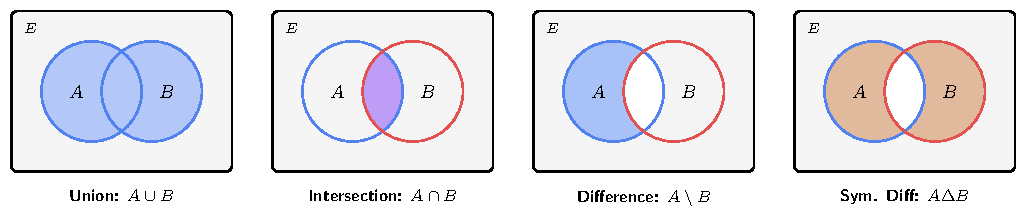
\includegraphics[width=0.95\textwidth]{01_venn_operations.pdf}
  \caption{\textbf{Fundamental Set Operations:} Geometric Venn diagram representation of Union ($A \cup B$), Intersection ($A \cap B$), Difference ($A \setminus B$), and Symmetric Difference ($A \Delta B$).}
  \label{fig:venn}
\end{figure}

\begin{definitionbox}{Fundamental Set Operations}
Let $A, B \in \mathcal{P}(E)$ be subsets of an ambient set $E$:
\begin{enumerate}[leftmargin=1.4em,itemsep=3pt]
  \item \textbf{Union:} $A \cup B = \{ x \in E \mid x \in A \lor x \in B \}$.
  \item \textbf{Intersection:} $A \cap B = \{ x \in E \mid x \in A \land x \in B \}$. If $A \cap B = \emptyset$, $A$ and $B$ are \textbf{disjoint}.
  \item \textbf{Set Difference (Relative Complement):} $A \setminus B = \{ x \in E \mid x \in A \land x \notin B \}$.
  \item \textbf{Complement in $E$:} $\complement_E A = E \setminus A = \{ x \in E \mid x \notin A \}$.
  \item \textbf{Symmetric Difference:} $A \Delta B = (A \setminus B) \cup (B \setminus A) = (A \cup B) \setminus (A \cap B)$.
  \item \textbf{Cartesian Product:} $A \times B = \{ (a, b) \mid a \in A \land b \in B \}$.
\end{enumerate}
\end{definitionbox}

\begin{theorembox}{De Morgan's Laws for Sets}
For any subsets $A, B \subseteq E$:
\begin{equation}
\complement_E (A \cup B) = \complement_E A \cap \complement_E B, \qquad \complement_E (A \cap B) = \complement_E A \cup \complement_E B.
\end{equation}
More generally, for any indexed family of subsets $\{A_i\}_{i \in I}$:
\begin{equation}
\complement_E \left( \bigcup_{i \in I} A_i \right) = \bigcap_{i \in I} \complement_E A_i, \qquad 
\complement_E \left( \bigcap_{i \in I} A_i \right) = \bigcup_{i \in I} \complement_E A_i.
\end{equation}
\end{theorembox}

\section{Worked Examples with Step-by-Step Proofs}

\begin{workedexample}{Irrationality of $\sqrt{2}$ by Contradiction}
Prove by contradiction that $\sqrt{2}$ is not a rational number ($\sqrt{2} \notin \mathbb{Q}$).

\paragraph{Solution and Proof.}
Assume to the contrary that the negation is true: $\sqrt{2} \in \mathbb{Q}$.
By definition of the rational numbers $\mathbb{Q}$, there exist two integers $a, b \in \mathbb{Z}$ with $b \neq 0$ such that:
\[
\sqrt{2} = \frac{a}{b}.
\]
Without loss of generality, we assume the fraction is in \textbf{irreducible form}, meaning that $\gcd(a, b) = 1$ ($a$ and $b$ share no common positive divisor other than $1$).

Squaring both sides of the equation:
\[
2 = \frac{a^2}{b^2} \implies a^2 = 2 b^2.
\]
This equation implies that $a^2$ is an even integer (a multiple of $2$).
\begin{itemize}[leftmargin=1.4em,itemsep=2pt]
  \item \textit{Lemma:} If $a^2$ is even, then $a$ is even.
  \item \textit{Proof of Lemma by Contrapositive:} Suppose $a$ is odd. Then $a = 2k + 1$ for some $k \in \mathbb{Z}$.
  Squaring gives $a^2 = (2k+1)^2 = 4k^2 + 4k + 1 = 2(2k^2 + 2k) + 1$, which is odd. Since the contrapositive holds, the lemma is established.
\end{itemize}
Because $a$ is even, there exists an integer $k \in \mathbb{Z}$ such that $a = 2k$.
Substituting $a = 2k$ back into our equation $a^2 = 2 b^2$:
\[
(2k)^2 = 2 b^2 \implies 4k^2 = 2 b^2 \implies b^2 = 2k^2.
\]
By the exact same reasoning, $b^2$ is even, which implies that $b$ must also be an even integer.

We have thus deduced that \textbf{both $a$ and $b$ are even}, meaning that $2$ divides both $a$ and $b$ ($2 \mid \gcd(a, b)$).
This directly contradicts our initial hypothesis that $\gcd(a, b) = 1$.
Therefore, the initial assumption that $\sqrt{2} \in \mathbb{Q}$ is false, concluding the proof that:
\[
\mathbf{\sqrt{2} \notin \mathbb{Q}}. \quad \blacksquare
\]
\end{workedexample}

\begin{workedexample}{Proof by Induction: Sum of the First $n$ Cubes}
Prove by mathematical induction that for every positive integer $n \ge 1$:
\[
\sum_{k=1}^n k^3 = 1^3 + 2^3 + 3^3 + \dots + n^3 = \left[ \frac{n(n+1)}{2} \right]^2.
\]

\paragraph{Solution and Proof.}
Let $P(n)$ be the proposition: $\sum_{k=1}^n k^3 = \left[ \frac{n(n+1)}{2} \right]^2$.

\textbf{1. Base Step ($n = 1$):}
For $n = 1$:
\[
\text{Left-Hand Side (LHS)} = 1^3 = 1.
\]
\[
\text{Right-Hand Side (RHS)} = \left[ \frac{1(1+1)}{2} \right]^2 = \left[ \frac{2}{2} \right]^2 = 1^2 = 1.
\]
Since $\mathrm{LHS} = \mathrm{RHS} = 1$, $P(1)$ is true.

\textbf{2. Inductive Step:}
Let $m \ge 1$ be an arbitrary integer. Assume that $P(m)$ is true (Induction Hypothesis):
\[
\sum_{k=1}^m k^3 = \left[ \frac{m(m+1)}{2} \right]^2.
\]
We must show that $P(m+1)$ is true, namely:
\[
\sum_{k=1}^{m+1} k^3 = \left[ \frac{(m+1)(m+2)}{2} \right]^2.
\]
Starting from the definition of the sum of $m+1$ terms:
\[
\sum_{k=1}^{m+1} k^3 = \left( \sum_{k=1}^m k^3 \right) + (m+1)^3.
\]
Substituting the Induction Hypothesis:
\[
\sum_{k=1}^{m+1} k^3 = \left[ \frac{m(m+1)}{2} \right]^2 + (m+1)^3 = \frac{m^2 (m+1)^2}{4} + (m+1)^3.
\]
Factoring out the common factor $(m+1)^2$:
\begin{align*}
\sum_{k=1}^{m+1} k^3 &= (m+1)^2 \left[ \frac{m^2}{4} + (m+1) \right] = (m+1)^2 \left[ \frac{m^2 + 4m + 4}{4} \right] \\
                    &= (m+1)^2 \left[ \frac{(m+2)^2}{4} \right] = \left[ \frac{(m+1)(m+2)}{2} \right]^2.
\end{align*}
This is precisely the statement $P(m+1)$.

\textbf{3. Conclusion:}
By the Principle of Mathematical Induction, the identity holds for all integers $n \ge 1$:
\[
\mathbf{\sum_{k=1}^n k^3 = \left[ \frac{n(n+1)}{2} \right]^2 = \left( \sum_{k=1}^n k \right)^2}. \quad \blacksquare
\]
\end{workedexample}

\begin{workedexample}{Rigorous Proof of De Morgan's Law for Sets}
Let $A$ and $B$ be two subsets of a universal set $E$. Prove rigorously by double inclusion that:
\[
\complement_E (A \cap B) = \complement_E A \cup \complement_E B.
\]

\paragraph{Solution and Proof.}
To establish set equality, we must prove two inclusions:
\begin{enumerate}[leftmargin=1.4em,itemsep=3pt]
  \item \textbf{Inclusion 1: $\complement_E (A \cap B) \subseteq \complement_E A \cup \complement_E B$.}
  Let $x \in \complement_E (A \cap B)$ be an arbitrary element.
  By definition of set complement:
  \[
  x \in E \quad \text{and} \quad x \notin (A \cap B).
  \]
  The statement $x \notin (A \cap B)$ is the logical negation of $x \in (A \cap B)$:
  \[
  \neg (x \in A \land x \in B).
  \]
  Applying De Morgan's logical law for conjunction:
  \[
  \neg (x \in A) \lor \neg (x \in B) \iff (x \notin A) \lor (x \notin B).
  \]
  Since $x \in E$, this translates to:
  \[
  (x \in E \land x \notin A) \lor (x \in E \land x \notin B) \iff x \in \complement_E A \lor x \in \complement_E B.
  \]
  By definition of set union:
  \[
  x \in (\complement_E A \cup \complement_E B).
  \]
  Since this holds for every $x \in \complement_E (A \cap B)$, we have established:
  \[
  \complement_E (A \cap B) \subseteq \complement_E A \cup \complement_E B.
  \]

  \item \textbf{Inclusion 2: $\complement_E A \cup \complement_E B \subseteq \complement_E (A \cap B)$.}
  Let $y \in (\complement_E A \cup \complement_E B)$ be an arbitrary element.
  By definition of union:
  \[
  y \in \complement_E A \lor y \in \complement_E B \iff (y \in E \land y \notin A) \lor (y \in E \land y \notin B).
  \]
  Thus $y \in E$ and $(y \notin A \lor y \notin B)$.
  By De Morgan's logical law, $(y \notin A \lor y \notin B) \iff \neg(y \in A \land y \in B) \iff y \notin (A \cap B)$.
  Therefore:
  \[
  y \in E \quad \text{and} \quad y \notin (A \cap B) \implies y \in \complement_E (A \cap B).
  \]
  This establishes the reverse inclusion:
  \[
  \complement_E A \cup \complement_E B \subseteq \complement_E (A \cap B).
  \]
\end{enumerate}
Combining both inclusions proves the identity:
\[
\mathbf{\complement_E (A \cap B) = \complement_E A \cup \complement_E B}. \quad \blacksquare
\]
\end{workedexample}

\begin{workedexample}{Characteristic Functions and Set Algebra}
For any subset $A \subseteq E$, its \textbf{characteristic function} (or indicator) is defined as:
\[
\mathbf{1}_A : E \longrightarrow \{0, 1\}, \qquad \mathbf{1}_A(x) = \begin{cases} 1 & \text{if } x \in A, \\ 0 & \text{if } x \notin A. \end{cases}
\]
\begin{enumerate}[leftmargin=1.4em,itemsep=2pt]
  \item Prove that for any two subsets $A, B \subseteq E$:
  \[
  \mathbf{1}_{A \cap B} = \mathbf{1}_A \cdot \mathbf{1}_B, \qquad \mathbf{1}_{\complement_E A} = 1 - \mathbf{1}_A.
  \]
  \item Using characteristic functions, derive the formula for the symmetric difference $\mathbf{1}_{A \Delta B}$.
\end{enumerate}

\paragraph{Solution and Proof.}
\textbf{1. Intersection and Complement:}
\begin{itemize}[leftmargin=1.4em,itemsep=2pt]
  \item For intersection: An element $x \in A \cap B \iff (x \in A \land x \in B)$.
  Thus $\mathbf{1}_{A \cap B}(x) = 1 \iff \mathbf{1}_A(x) = 1 \land \mathbf{1}_B(x) = 1 \iff \mathbf{1}_A(x) \cdot \mathbf{1}_B(x) = 1 \times 1 = 1$.
  If $x \notin A \cap B$, at least one of $\mathbf{1}_A(x)$ or $\mathbf{1}_B(x)$ is $0$, making the product $0$.
  Thus $\mathbf{1}_{A \cap B} = \mathbf{1}_A \cdot \mathbf{1}_B$.
  \item For complement: If $x \in \complement_E A$, then $x \notin A \implies \mathbf{1}_A(x) = 0$, so $1 - \mathbf{1}_A(x) = 1 - 0 = 1 = \mathbf{1}_{\complement_E A}(x)$.
  If $x \in A$, then $\mathbf{1}_A(x) = 1$, so $1 - \mathbf{1}_A(x) = 1 - 1 = 0 = \mathbf{1}_{\complement_E A}(x)$.
  Thus $\mathbf{1}_{\complement_E A} = 1 - \mathbf{1}_A$.
\end{itemize}

\textbf{2. Symmetric Difference $\mathbf{1}_{A \Delta B}$:}
Recall that $A \Delta B = (A \setminus B) \cup (B \setminus A) = (A \cap \complement_E B) \cup (B \cap \complement_E A)$.
Notice that $A \cap \complement_E B$ and $B \cap \complement_E A$ are strictly disjoint sets.
For any two disjoint sets $X$ and $Y$ ($X \cap Y = \emptyset$), $\mathbf{1}_{X \cup Y} = \mathbf{1}_X + \mathbf{1}_Y$.
Therefore:
\begin{align*}
\mathbf{1}_{A \Delta B} &= \mathbf{1}_{A \cap \complement_E B} + \mathbf{1}_{B \cap \complement_E A} \\
                       &= \mathbf{1}_A \cdot \mathbf{1}_{\complement_E B} + \mathbf{1}_B \cdot \mathbf{1}_{\complement_E A} \\
                       &= \mathbf{1}_A(1 - \mathbf{1}_B) + \mathbf{1}_B(1 - \mathbf{1}_A) \\
                       &= \mathbf{1}_A - \mathbf{1}_A \mathbf{1}_B + \mathbf{1}_B - \mathbf{1}_A \mathbf{1}_B \\
                       &= \mathbf{\mathbf{1}_A + \mathbf{1}_B - 2 \mathbf{1}_A \mathbf{1}_B} = (\mathbf{1}_A - \mathbf{1}_B)^2.
\end{align*}
This remarkable algebraic correspondence transforms boolean set manipulations directly into standard polynomial arithmetic!
\end{workedexample}
